%!TEX root =  ../paper.tex


\ifusenix
\begin{figure}[t]
 \centering
  %\includegraphics[trim={0 10.5cm 19cm 0},clip,width=0.75\linewidth]{ApproachRevised_2.pdf}
  %\includegraphics[trim={0 11.2cm 19cm 0},clip,width=0.75\linewidth]{ApproachRevised_3.pdf}
  \includegraphics[trim={0 11cm 19.2cm 0},clip,width=0.70\linewidth]{ApproachRevised_4.pdf}
 \caption{\textbf{Approach overview.} A trusted embedded device \device is attached to the target platform, verifies the proximity of the attested enclave, and enables a secure connection to it.}
 \vspace{-15px}
 \label{fig:approach}
\end{figure}

\else

\begin{figure}[t]
 \centering
  %\includegraphics[trim={0 10.5cm 19cm 0},clip,width=0.75\linewidth]{ApproachRevised_2.pdf}
  %\includegraphics[trim={0 11.2cm 19cm 0},clip,width=0.75\linewidth]{ApproachRevised_3.pdf}
  \includegraphics[trim={0 11cm 19.2cm 0},clip,width=0.45\linewidth]{ApproachRevised_4.pdf}
 \caption{\textbf{Approach overview.} A trusted embedded device \device is attached to the target platform, verifies the proximity of the attested enclave, and enables a secure connection to it.}
 %\vspace{-20px}
 \label{fig:approach}
\end{figure}
\fi

\section{\name Attestation}
\label{sec:ourApproach}

The goal in this chapter is to design a solution that addresses the above limitations of previous solutions. In short, our solution should be \emph{secure} (small TCB, no online authorities) and \emph{easy to deploy} (no OS re-installation, manual configuration or pre-defined enclaves). In this section, we provide an overview of our approach and then describe two novel solution variants.

%We start with an overview, explain our security assumptions, then outline example use cases, and finally present our two attestation variants.
% \emph{Distance-Bounding} and \emph{Boot-Time initialization}.

\subsection{Approach Overview}

We propose a hardened SGX attestation scheme, called \name, based on a simple and auxiliary embedded device that we call \device. %\footnote{We note that the idea of proximity verification for remote attestation has been proposed in the previous literature in the context of TPM attestation (see, e.g.,~\cite{CatchingCuckoo,turtle}), but never realized as a fully-functional system. In Section~\ref{sec:relatedWork} we review these previous works in more detail.}
The embedded device is attached to the target platform over a local communication interface, such as USB, as shown in  Figure~\ref{fig:approach}. Using this approach, we propose two hardened attestation mechanism to address the relay and emulation attackers defined in Section~\ref{sec:problemStatement:attackerModel}.


\blue{Our first attestation mechanism prevents relay attacks. The main idea in this mechanism is \emph{proximity verification}: \device verifies the proximity of the attested enclave and after successful proximity verification it facilitates the creation of a secure channel between the remote verifier and the attested enclave. This mechanism is described in Section~\ref{sec:systemDesign}.} 

\blue{Our second attestation mechanism is designed to prevents emulation attacks. The main idea in this mechanism is \emph{boot-time initialization}. We bootstrap a secure connection between \device and a specialized enclave by booting the platform from a minimal OS kernel from the \device. This specialized enclave later executes local attestation to other application-specific enclaves on the standard OS. This mechanism is described in Section~\ref{sec:variantII}.}

In both of our attestation mechanisms, the \device device periodically checks proximity to the attested enclave. The established secure channel is contingent on the physical presence of the embedded device on the target machine and it stays active only as long as the device is plugged-in. The act of detaching the device automatically revokes the attested platform without any interaction with a trusted authority. Thus, our solution enables \propname. 

To use our solution, enclave developers add function calls to a simple \name API that facilitates communications between the enclave and the device (see Figure~\ref{fig:approach}).


\ifusenix
\vspace{-15pt}
\else
\fi
\myparagraph{Security assumptions.}
%\label{sec:ext-attacker-model}
The \device device is a trusted component in our solution. We deem this choice reasonable since it implements only the strictly necessary functions and therefore it a has significantly smaller software TCB, attack surface, and hardware complexity compared to the host OS. 
%and hypervisor solutions like~\cite{sgxio}.
%\todo{Mention that attacker may have leaked keys from other similar devices (extension of system and attacker model).}
We assume that its issuer certifies each embedded device prior to its deployment (such certification can take place fully offline). %\device has a public and private key hardcoded into it, and it can store the issuer's certificate for its public key.
%These keys are needed because, among other things, we need to be able to differentiate between different devices. The role of the keys embedded into \device will be discussed in more detail in the following sections.

Concerning the security of the \device device we employ the same attacker model introduced in Section~\ref{sec:problemStatement} for enclaves. While the user's device and its private keys are never exposed to the attacker, another similar device can be in the physical possession of the attacker, which has as much time as she wants to fully compromise it (run arbitrary code and extract keys). %Note that this model makes \device susceptible to relay as well as emulation attacks since given a \device private key the attacker can emulate that \device in any platform in which she controls the OS.

%Finally, we assume that the issuer of the embedded device can secure communicate the identity of the of the specific device to its user, that is, the remote verifier.


\subsection{Example Use Cases}
\label{sec:use-cases}

%\begin{figure}[t]
% \centering
%     %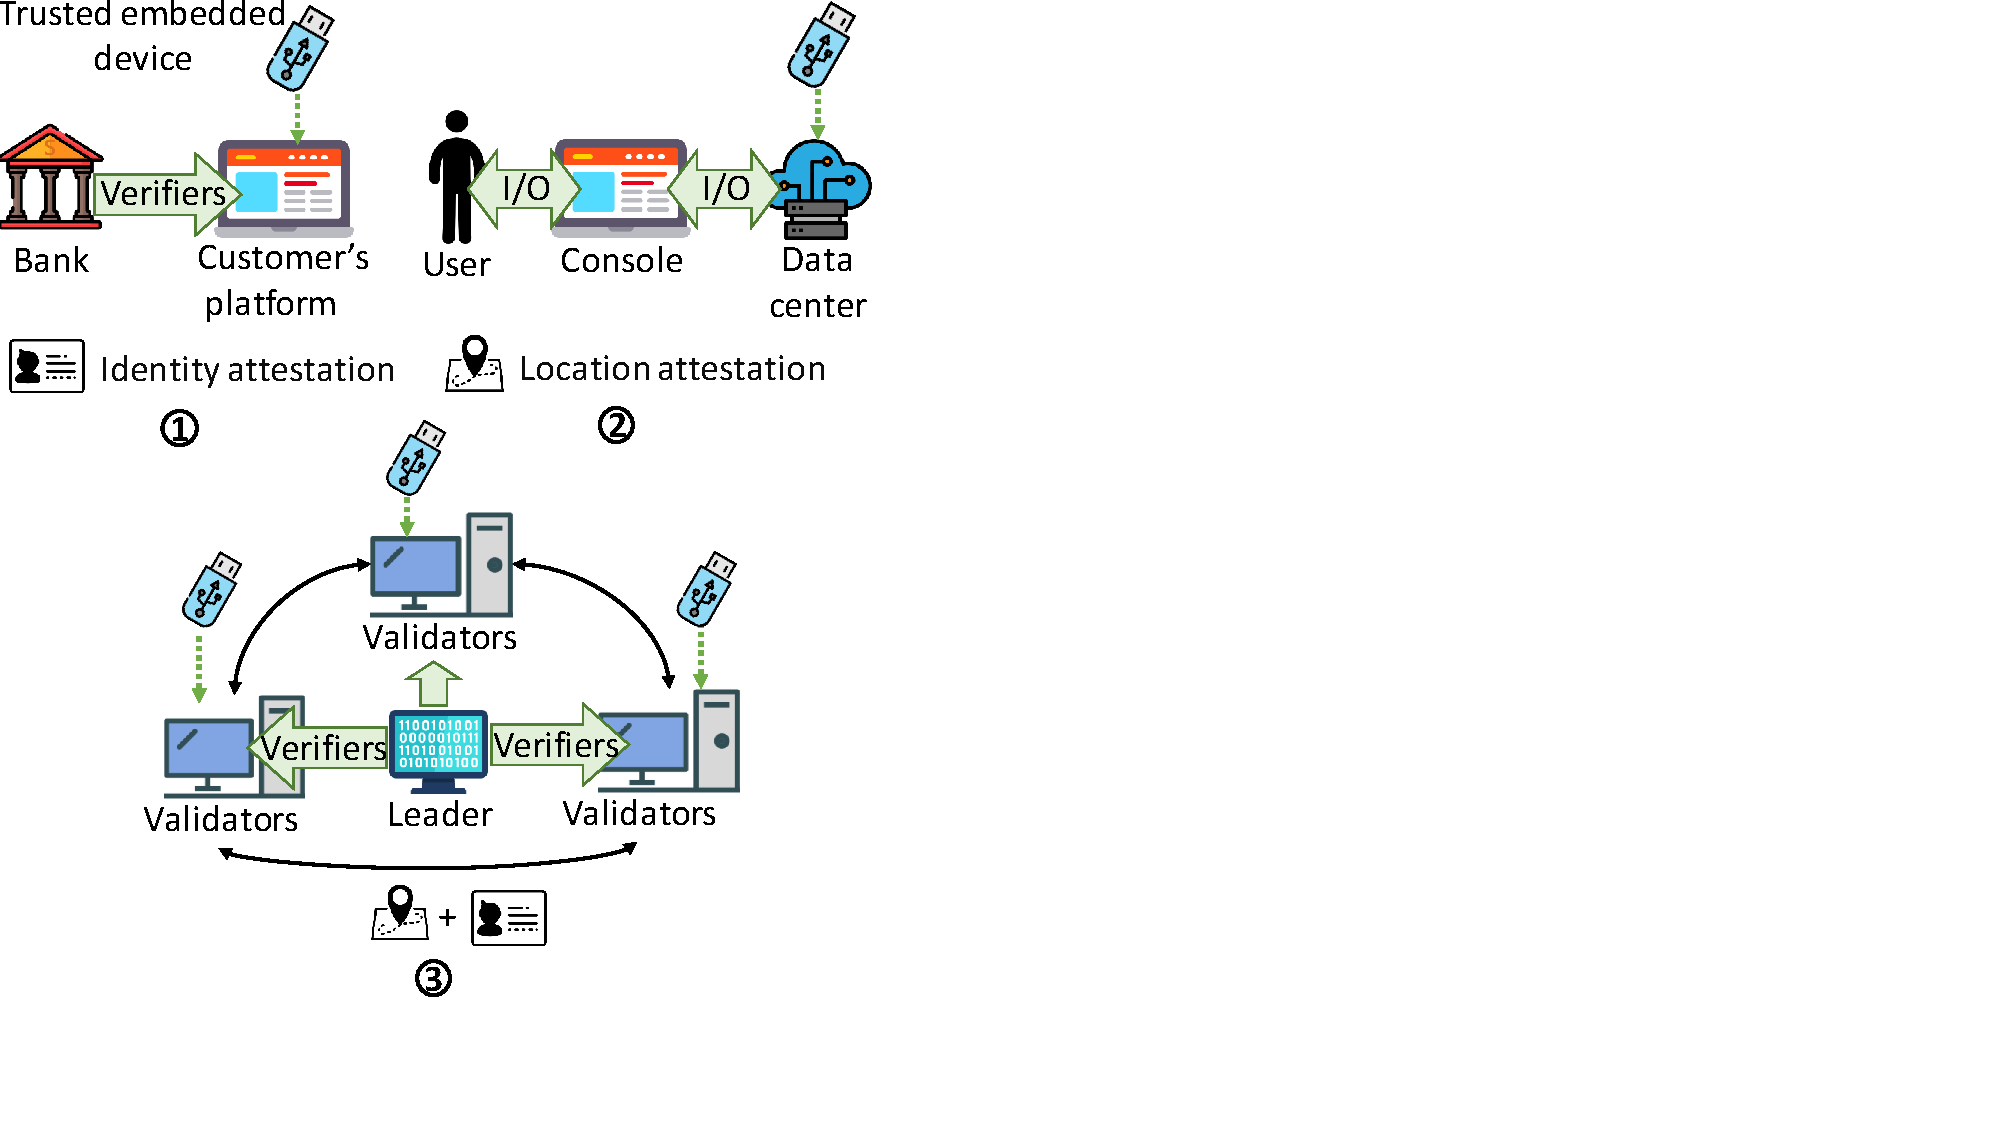
\includegraphics[trim={0 2.1cm 19.1cm 0},clip,width=0.45\linewidth]{UseCases_revised_1.pdf}
%     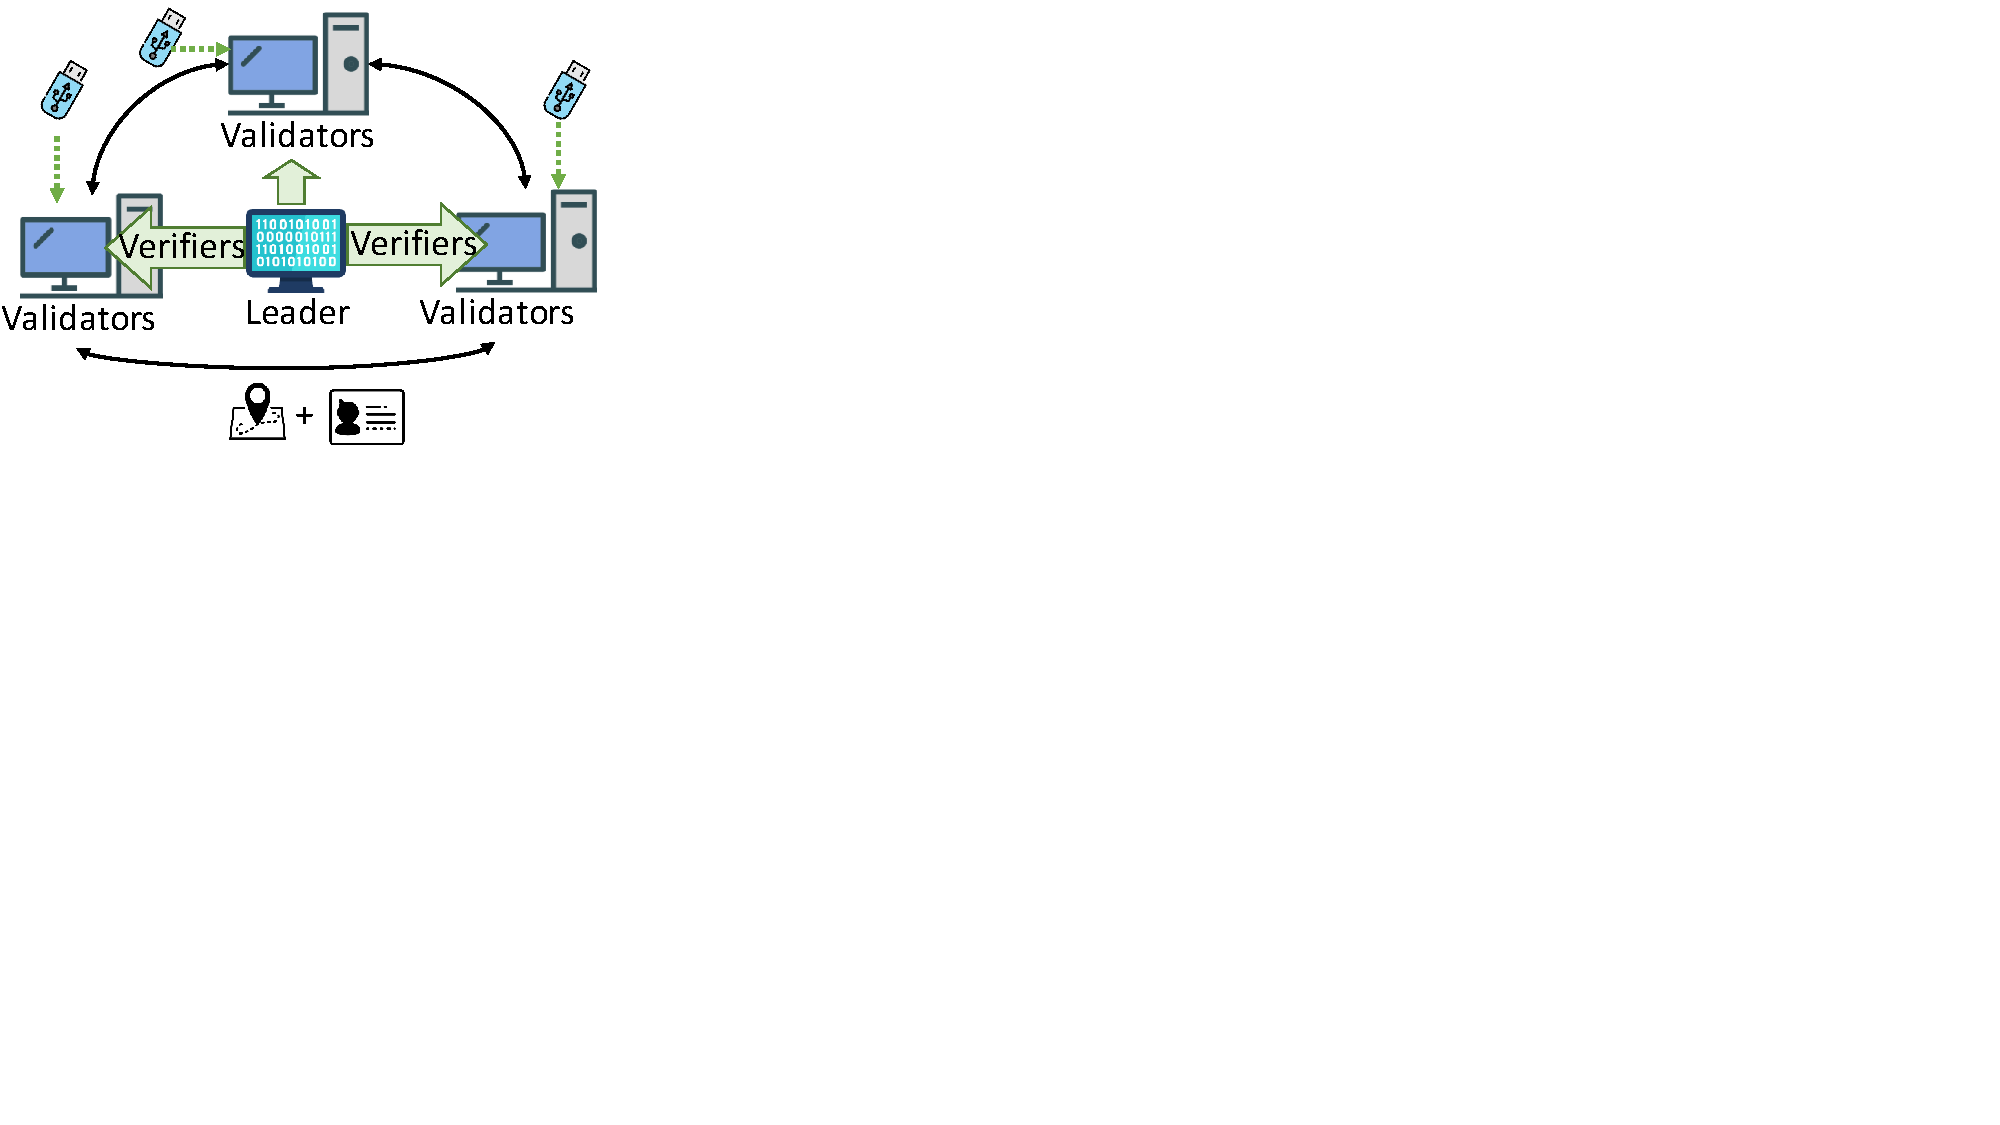
\includegraphics[trim={0 11.5cm 23.5cm 0},clip,width=0.3\linewidth]{UseCases_blockchain.pdf}
% %\caption{\textbf{Use cases and types of attestation.} \one Remote verifier such as bank checks if the platform from where the customer logs in is connected to the bank-issued embedded device. \two The user establishes a secure path to a TEE on the remote server like data center. \three Group leader verifies the TEEs for permissioned blockchain validator nodes.}
% 
% \caption{\textbf{\name in permissioned blockchain scenario.} \name strengthen SGX attestation by adding the notion of identity and location to it. Group leader verifies the TEEs for permissioned blockchain validator nodes.}
%%\vspace{-20pt}
% \label{fig:SystemSettings}
%\end{figure}

%Our solution is designed for deployments where the benefits of more secure attestation outweighs the deployment cost of a simple auxiliary device. Here, we briefly describe two such examples.  

Our solution is targeted to scenarios where the benefits of more secure attestation outweigh the deployment cost of a simple auxiliary device. Here, we outline two such examples.  

%\begin{mylist}
%  \item[\one] \emph{User identification in online services.} In the first use case, we consider a remote verifier such as a bank or a company. The remote verifier issues a certified \device to the owner of the attested target platform, such as a customer of a bank\footnote{Note that it is common for banks and to distribute hardware tokens to account holders, and by authenticating the user's input this new device could replace existing solutions.} or an employee of a company. We call this type of attestation \emph{identity-based attestation} as it enables the remote verifier to verify the owner of the attested platform. Binding the user's identity to a computing platform can be realized by plugging in the trusted embedded device to the platform. Our approach guarantees the attested user can communicate with the bank if and only if the \device is physically attached to the user's platform. If the user switches to a new computing platform, the act of moving \device to the new platform automatically revokes the old platform.

  %\item[\two] \emph{Outsourcing data to remote infrastructures.} In the second use case, the issuer of the trusted embedded device also physically enforces the location in which it can be deployed. For instance, a 
  Our first example is cloud platform provider that attaches \device to a server in a specific data center and makes the public key of the attached device known to the users of the service. Our approach is especially well suited to cloud computing models where customers rent dedicated computing resources like entire servers. In such setting, our solution ensures that the cloud platform customer outsources data and computation to a server that resides in a specified location. Enforcing location may be desirable to meet increasing data protection regulation that defines how and where data can be stored, even if protected by TEEs such as SGX. Revocation (e.g., when a server is relocated to another data center or function) can be realized by merely detaching \device.

%  \item[\three] \emph{Initialization of permissioned blockchains.} As our third example we consider a 
Our second example is a trusted authority that initializes a set of validator nodes for a permissioned, SGX-hardened blockchain. 
%(see Figure~\ref{fig:SystemSettings})
The trusted authority issues one \device device for each organization that operates one of the validator nodes which allows secure attestation of the validator platforms. Organizations are free to upgrade their computing platforms by attaching the \device to a new platform which automatically revokes the old platform without the need to interact with the trusted authority. Furthermore, since \device can only be active on one platform at the time, such a deployment enables the trusted authority to bound the ``voting power'' (e.g., identities in Byzantine consensus) of each validator organization in the blockchain consensus.
  %on the amount of computational resources each validator can make use of, and other validators to check that the bound is enforced.
%\end{mylist}



\subsection{\blue{Addressing Relay Attacks}}
\label{sec:systemDesign}

\blue{Now we described our first hardened attestation mechanism that is designed to prevent relay attacks.} The main idea behind is to use the \device device to perform both a standard remote attestation and then verify the proximity of the attested enclave using distance bounding. If both steps succeed, the embedded device enables the remote verifier to establish a secure connection to the enclave.

\ifusenix
\vspace{-15pt}
\else
\fi
\myparagraph{Attestation protocol.} Figure~\ref{fig:systemSetUp} illustrates the attestation protocol that proceeds as follows:


\ifusenix

\begin{figure}[t]
 \centering
  %\includegraphics[trim={0 4.6cm 18cm 0},clip,width=0.5\linewidth]{SystemSetupRevised_3.pdf}
  \includegraphics[trim={0 8.8cm 13.2cm 0},clip,width=\linewidth]{SystemSetupRevised_5.pdf}
 \caption{\textbf{Attestation variant I: distance bounding.} The remote verifier establishes a secure channel to the \device embedded device that performs standard attestation and verifies the proximity of the attested using distance bounding.}
 \vspace{-2px}
 \label{fig:systemSetUp}
\end{figure}

\begin{figure}[t]
  \centering
    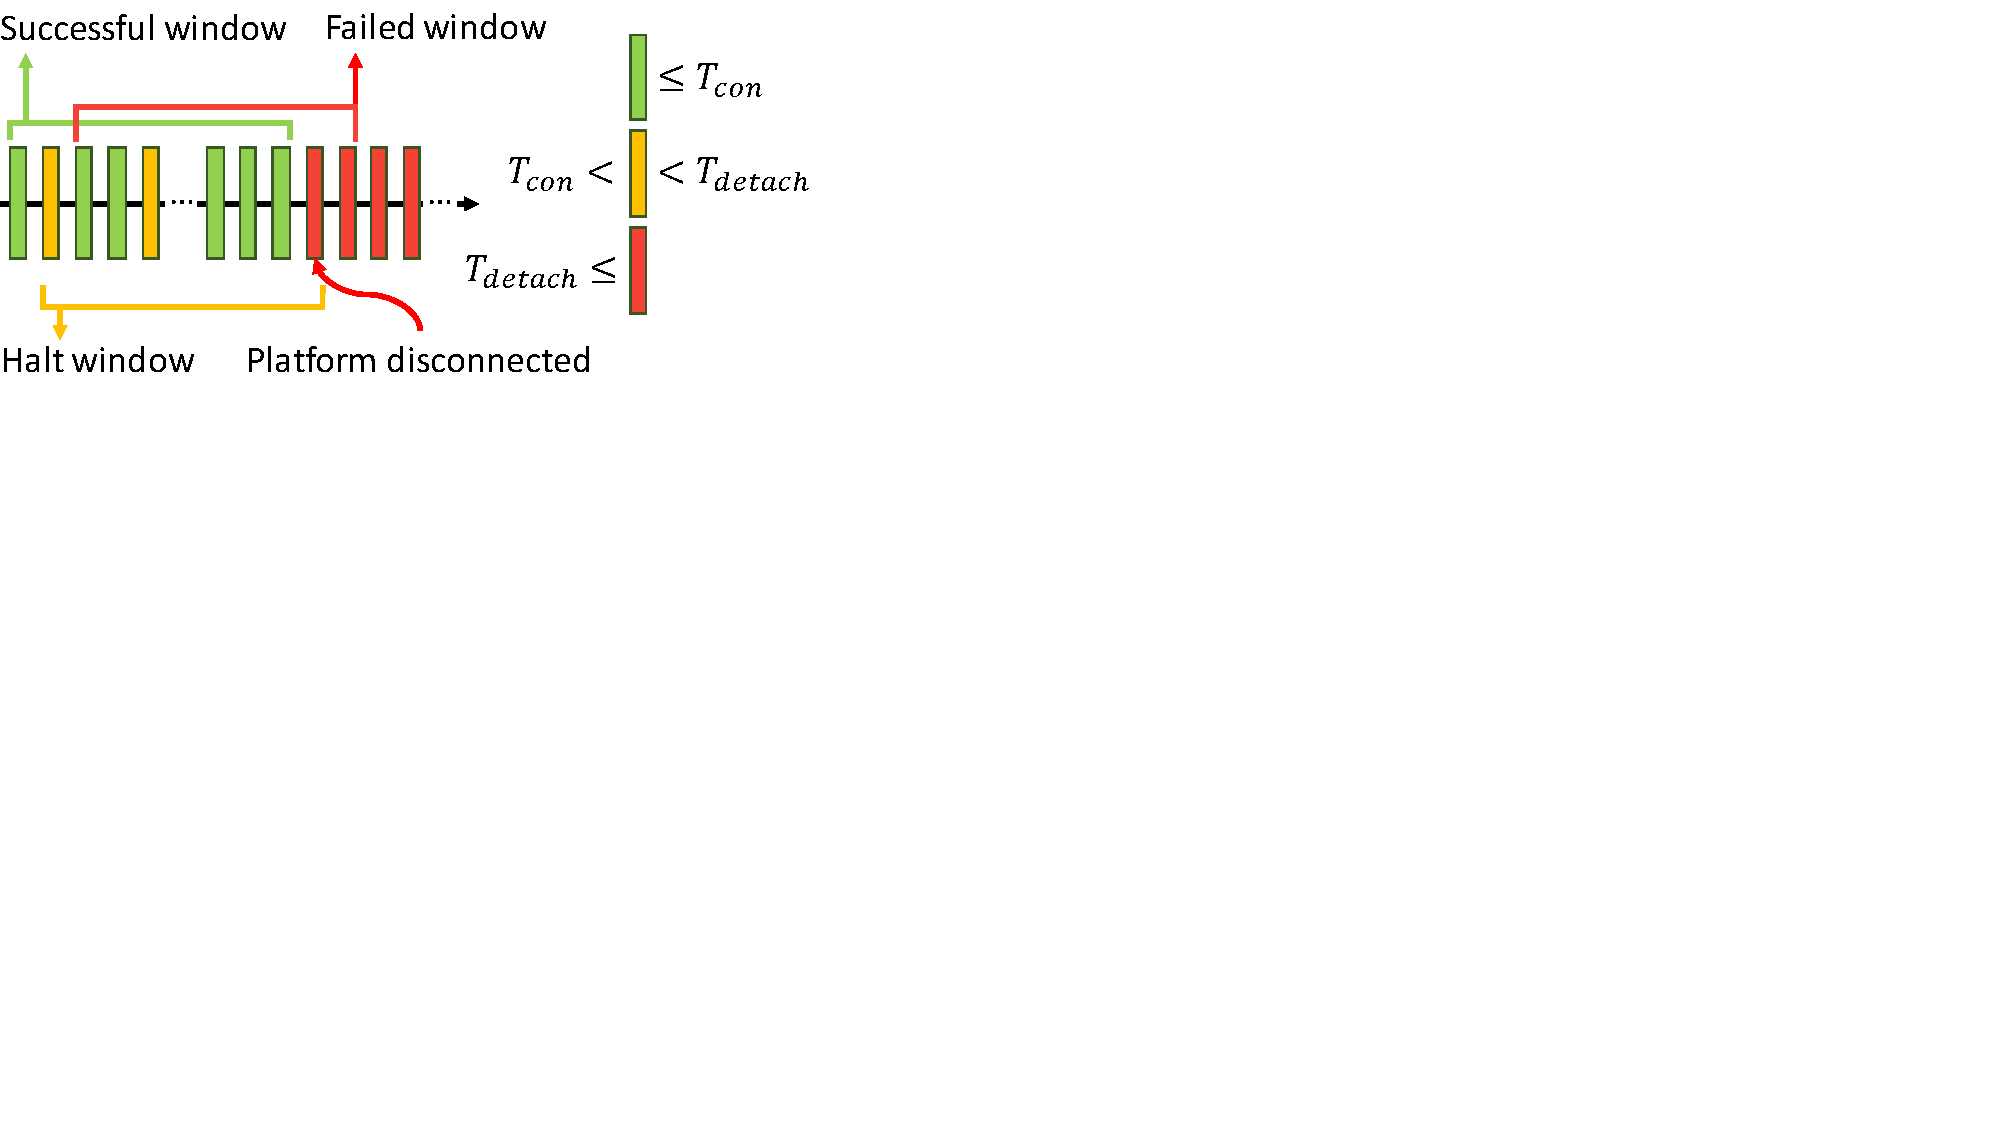
\includegraphics[trim={0 12.7cm 20cm 0}, clip, width=0.7\linewidth]{SlidingWindow.pdf}
    \caption{\textbf{Sliding window.} The figure shows an example of sliding windows for periodic proximity verification.}
    \vspace{-10px}
    \label{fig:slidingWindow}
\end{figure}

\else

\begin{figure*}[t!]
    \centering
    \begin{subfigure}[t]{0.6\textwidth}
        \centering
        \includegraphics[trim={0 4.6cm 18cm 0},clip, height=2.65in]{SystemSetupRevised_3.pdf}
        \caption{\textbf{Flow of distance bounding attestation.} The remote verifier establishes a secure channel to the \device embedded device that performs standard attestation and verifies the proximity of the attested using distance bounding.}
        \label{fig:systemSetUp}
    \end{subfigure}%
    ~ ~~
    \begin{subfigure}[t]{0.4\textwidth}
        \centering
        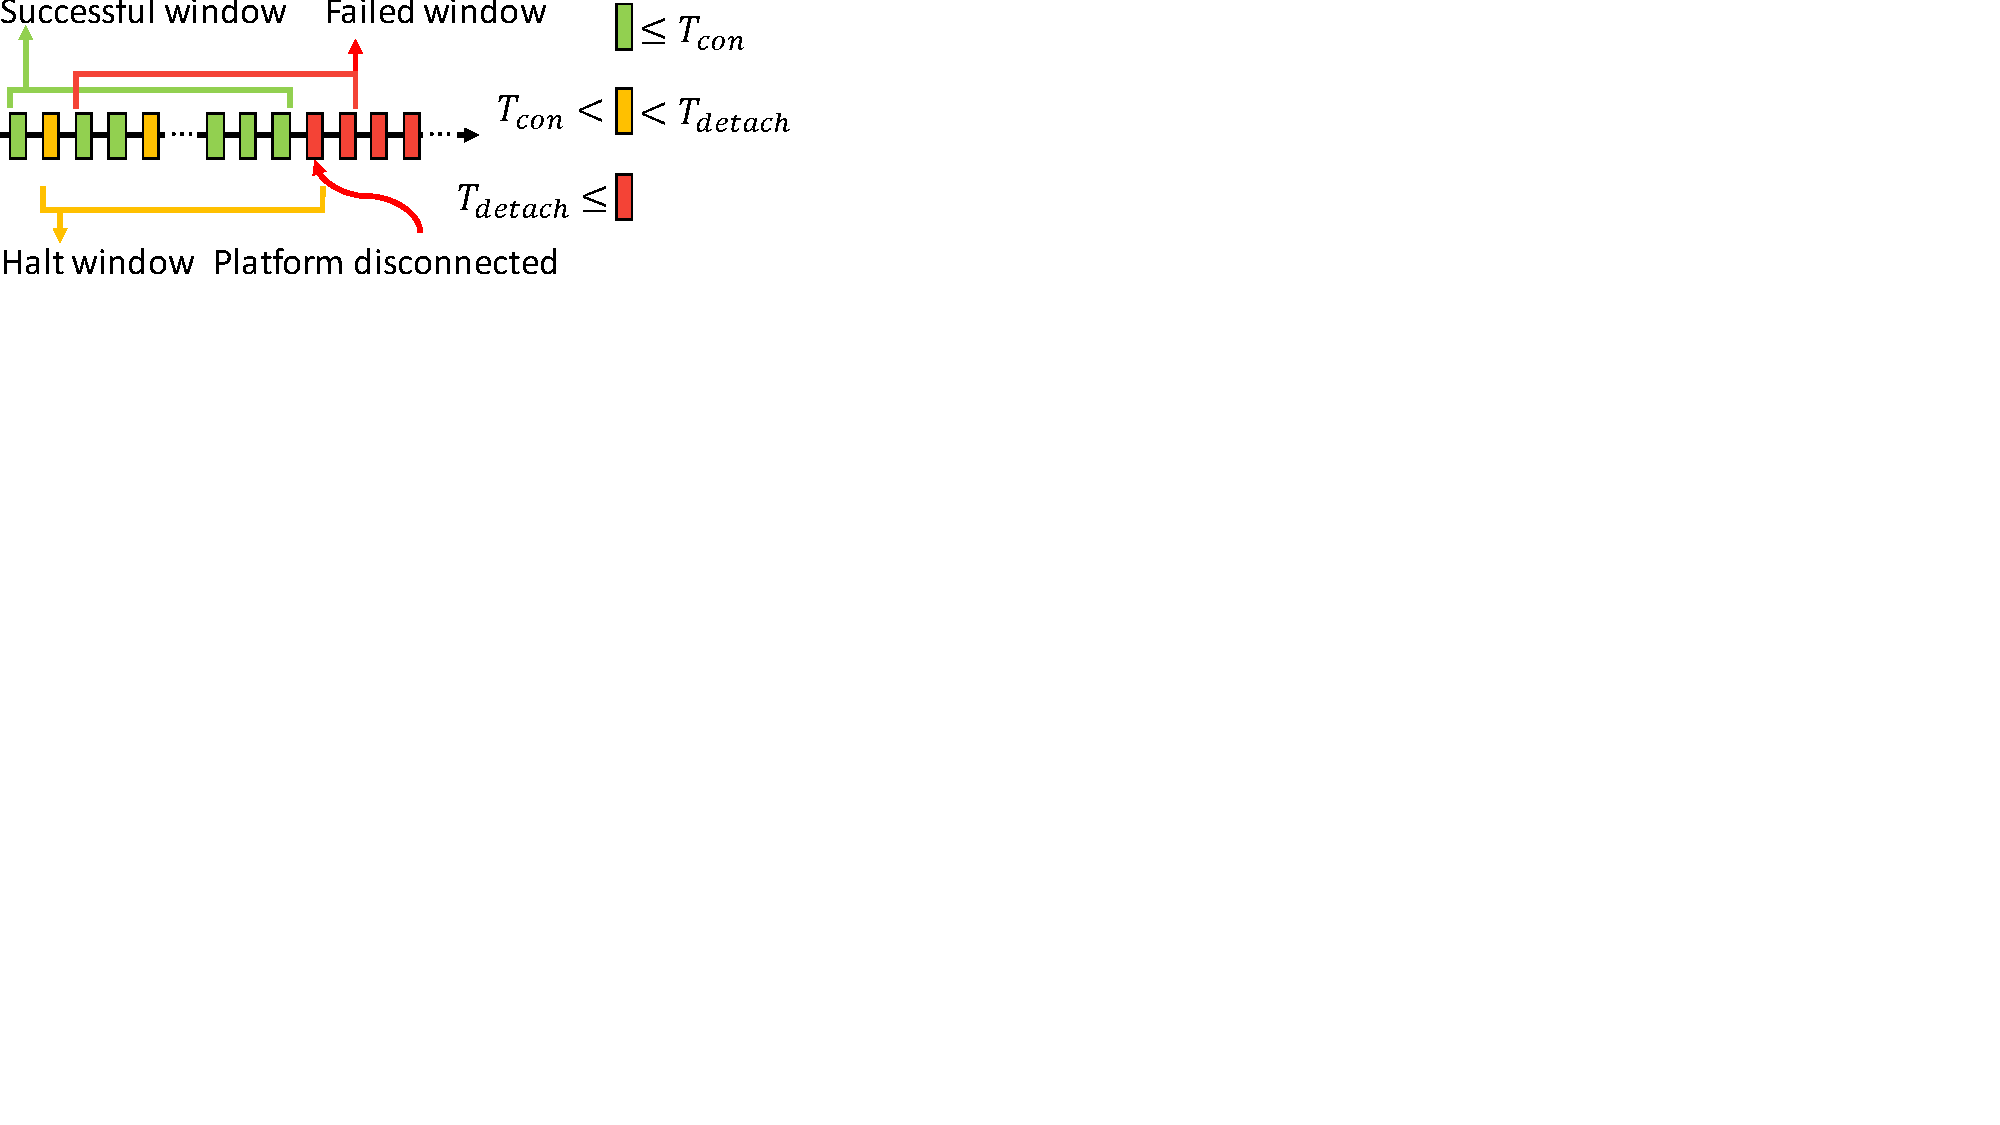
\includegraphics[trim={0 8cm 22cm 0}, clip, height=2.15in]{SlidingWindow_1.pdf}
        \caption{\textbf{Sliding window.} The figure shows an example of sliding windows for periodic proximity verification.}
        \label{fig:slidingWindow}
    \end{subfigure}
    \caption{\textbf{Attestation variant 1: distance bounding.}}
\end{figure*}


%\vspace{-6pt}

\fi

\begin{mylist}
  \item[\one] The remote verifier establishes a secure channel (e.g., \tls) to the certified \device. An assisting but untrusted user-space application facilitates the connection on the target platform acting as a transport channel between the remote verifier and the \device (and later also the enclave). As part of this first step, the remote verifier specifies which enclave should be executed.

  \item[\two] The untrusted application creates and starts the attestation target enclave.

  \item[\three] \device performs the standard remote attestation protocol to verify the code configuration of the enclave with the help of the IAS server (see Appendix~\ref{sec:background} for attestation protocol details). In the attestation protocol, the device learns the public key of the attested enclave.

  \item[\four] \device establishes a secure channel (e.g., \tls) to the enclave using that public key.

  \item[\five] \device performs a distance-bounding protocol that consists of $n$ rounds, where each round is formed by steps \five to \eight.
  %(see Figure~\ref{fig:challengeResponse}).
  At the beginning of each round \device generates a random challenge $r$ and sends it to the enclave over the TLS channel.

  \item[\six] The enclave increments the received challenge by one.

  \item[\seven] The enclave sends a response ($r+1$) back to the \device over the \tls channel.

  \item[\eight] \device verifies that the response value is as expected (i.e., $r+1$) and checks if the latency of the response is below a threshold (\connect). Successful proximity verification requires that the latency is below the threshold for a sufficient fraction ($k$, at least $k \times n$ out of $n$) of responses.

  \item[\nine] If proximity verification is successful, the \device notifies the remote verifier over the \tls channel (constructed in step \one). The verifier starts using the \device TLS channel to send messages to the enclave.

\end{mylist}



\ifusenix
\vspace{-14pt}
\else
\fi
\myparagraph{Periodic proximity verification.} After the initial connection establishment, the \device device performs \emph{periodic} proximity verification on the attested enclave. \device sends a new random challenge $r$ at frequency $f$, verifies the correctness of the received response and measures its latency. The latest $w$ latencies are stored to a sliding window data structure, as shown in Figure~\ref{fig:slidingWindow}.

As elaborated in Section~\ref{sec:evaluation} there are three types of latencies in the presence of relay attacks. The first type of response is received faster than the  threshold \connect (green in Figure~\ref{fig:slidingWindow}), these responses can only be produced if no attack is taking place. In the second type of response the latency exceeds \connect, but it is below another, higher threshold \detach (yellow), these are sometimes observed during legitimate connections and sometimes during relay attacks. And third, the latency is equal to or exceeds \detach (red), these latencies are only observed while a relay attack is being performed. Given such a sliding window of periodic challenge-response latencies, we define the following rules for halting or terminating the connection:

\begin{mylist}
  \item \textbf{Successful window: no action.} If at least $k$ responses have latency $\leq$\connect and none of the response have latency$\geq$\detach, we consider the current window legitimate. \device keeps the connection active (i.e., no action).
 
  \item \textbf{Halt window: prevent communication.} If one of the responses have latency $\geq$\detach, we consider the current window a ``halt window'' and \device stops forwarding further communication to the enclave until the current window is legitimate again.

  \item \textbf{Failed window: terminate channel.} If two or more responses have latencies $\geq$\detach, we consider the current window a ``failed window'' and \device terminates the communication and revokes the attested platform.
\end{mylist}


\iffalse
\myparagraph{Following communication.}
%Subsequently, to prevent he time of check vs. time of use (TOCTOU) problems,
After attestation, \device performs proximity verification with the attested enclave periodically at frequency $f$ (e.g., $f=1/s$). If the proximity verification fails, \device tries immediately again. If proximity verification fails a threshold $T$ number of times successively (e.g., $T=10$), \device determines that it must have been detached and it prevents further communication with the attested enclave. In Section~\ref{sec:evaluation} discuss parameter values for $f$ and $T$.
\fi

\subsection{\blue{Addressing Emulation Attacks}}
\label{sec:variantII}

\blue{Proximity verification alone cannot protect against emulation attacker, as \device cannot distinguish between the enclave running on the physical processor versus the enclave running on the emulated processor. Next, we describe our second hardened attestation mechanism that is designed to prevent emulation attacks as well. This solution can be seen as a novel variant of trust on first use that simplifies deployment (e.g., no OS reinstall or pre-defined enclaves) and increases security (e.g., small TCB, no online authorities).} %Additionally, usage of the trusted device enables additional properties such as offline revocation.

%Our solution is different from the simple and commonly suggested of TOFU approaches (see Section~\ref{sec:problemStatement:limitations}) in two ways. First, we enable improved deployability by reducing the OS reinstallation to platform reboot operation. Second, we leverage the attached embedded device to enable offline enrollment and revocation.


\ifusenix
\begin{figure}[t]
 \centering
%     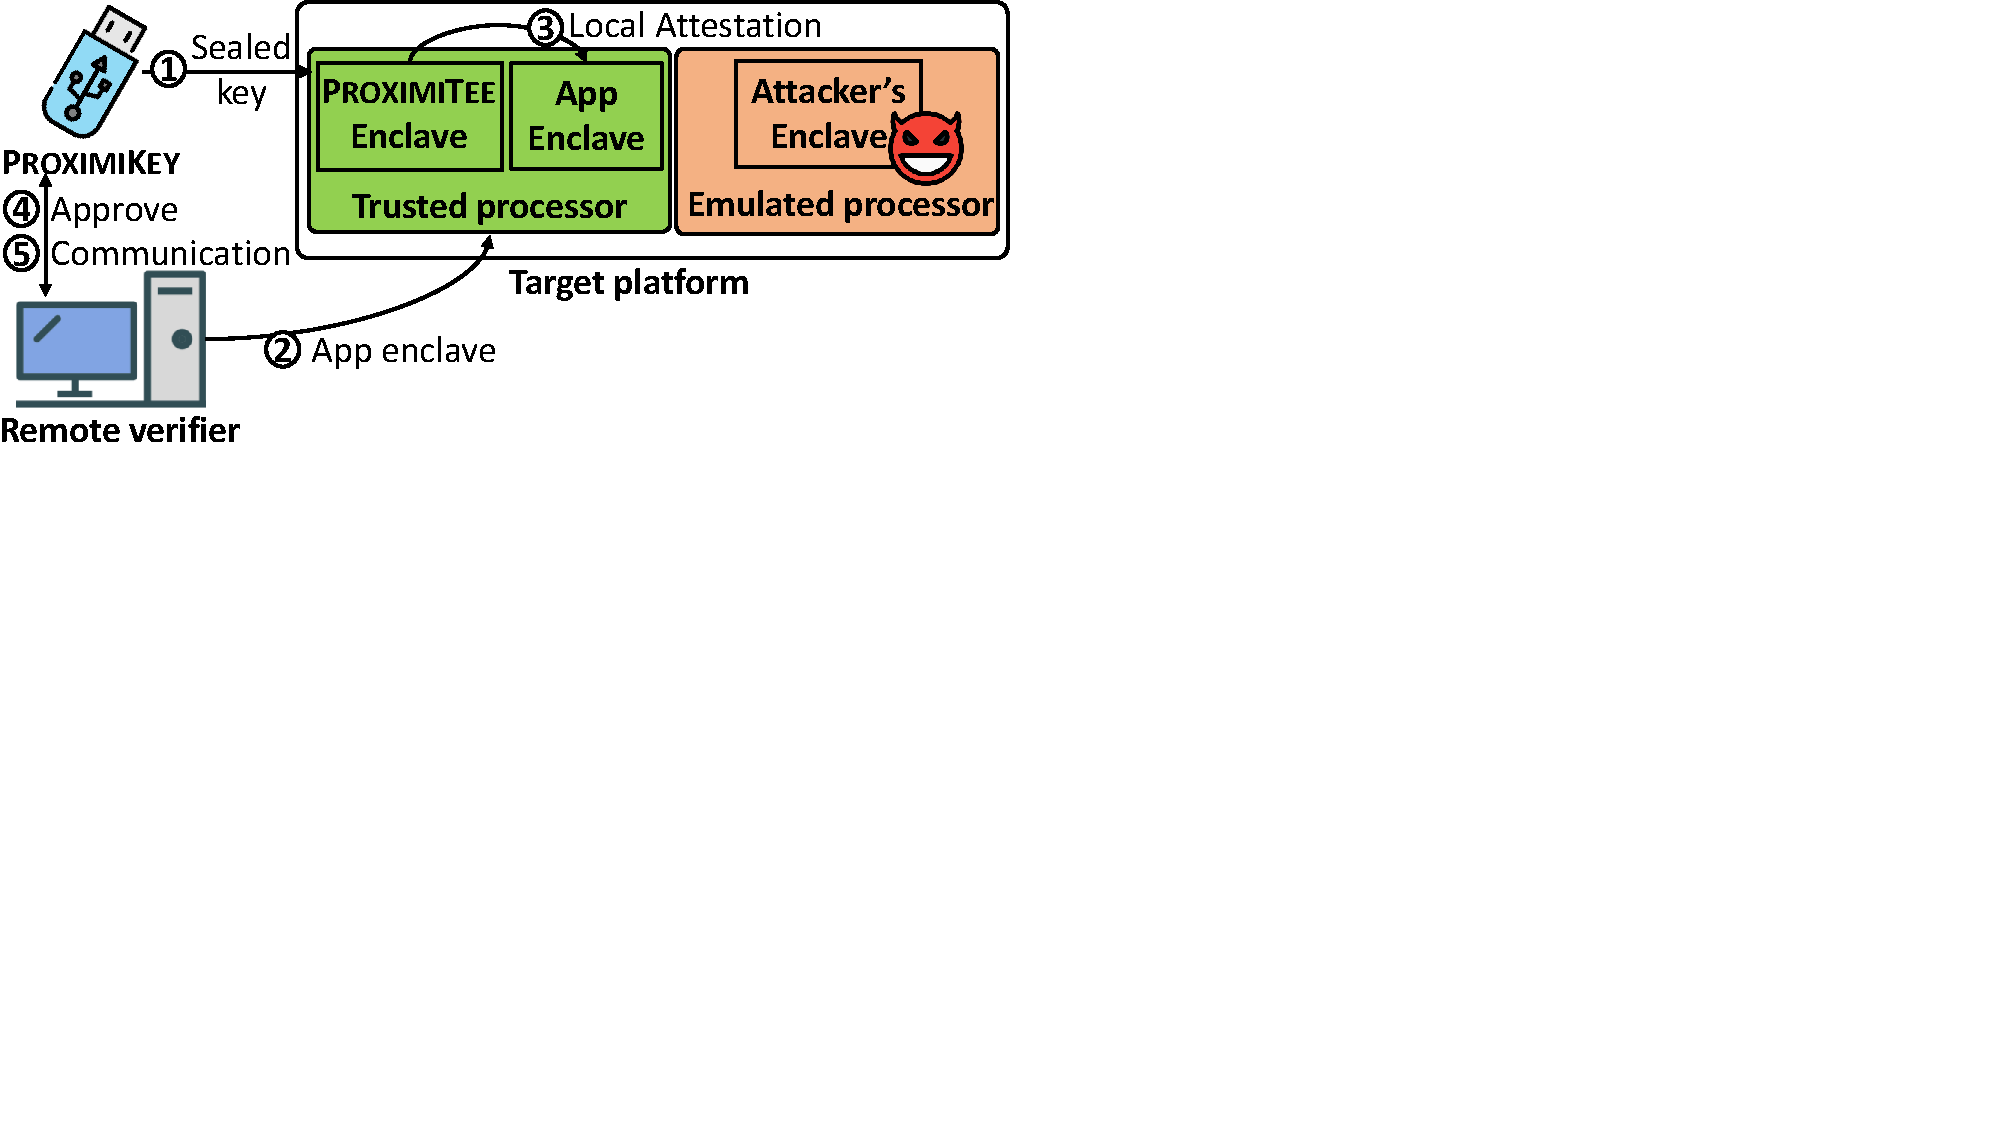
\includegraphics[trim={0 10cm 16.8cm 0},clip,width=0.8\linewidth]{boot-attest.pdf}
\includegraphics[trim={0 11.6cm 16.5cm 0},clip,width=0.75\linewidth]{boot-attest_2.pdf}
 \caption{\textbf{Attestation variant 2: boot-variant attestation.} After the boot-time initialization (refer to Figure~\ref{fig:boot-init}) the \nameclave executes a local attestation with the verifier uploaded \app. 
 }
\vspace{-5pt}
 \label{fig:boot-attest}
\end{figure}


\begin{figure}[t]
 \centering
    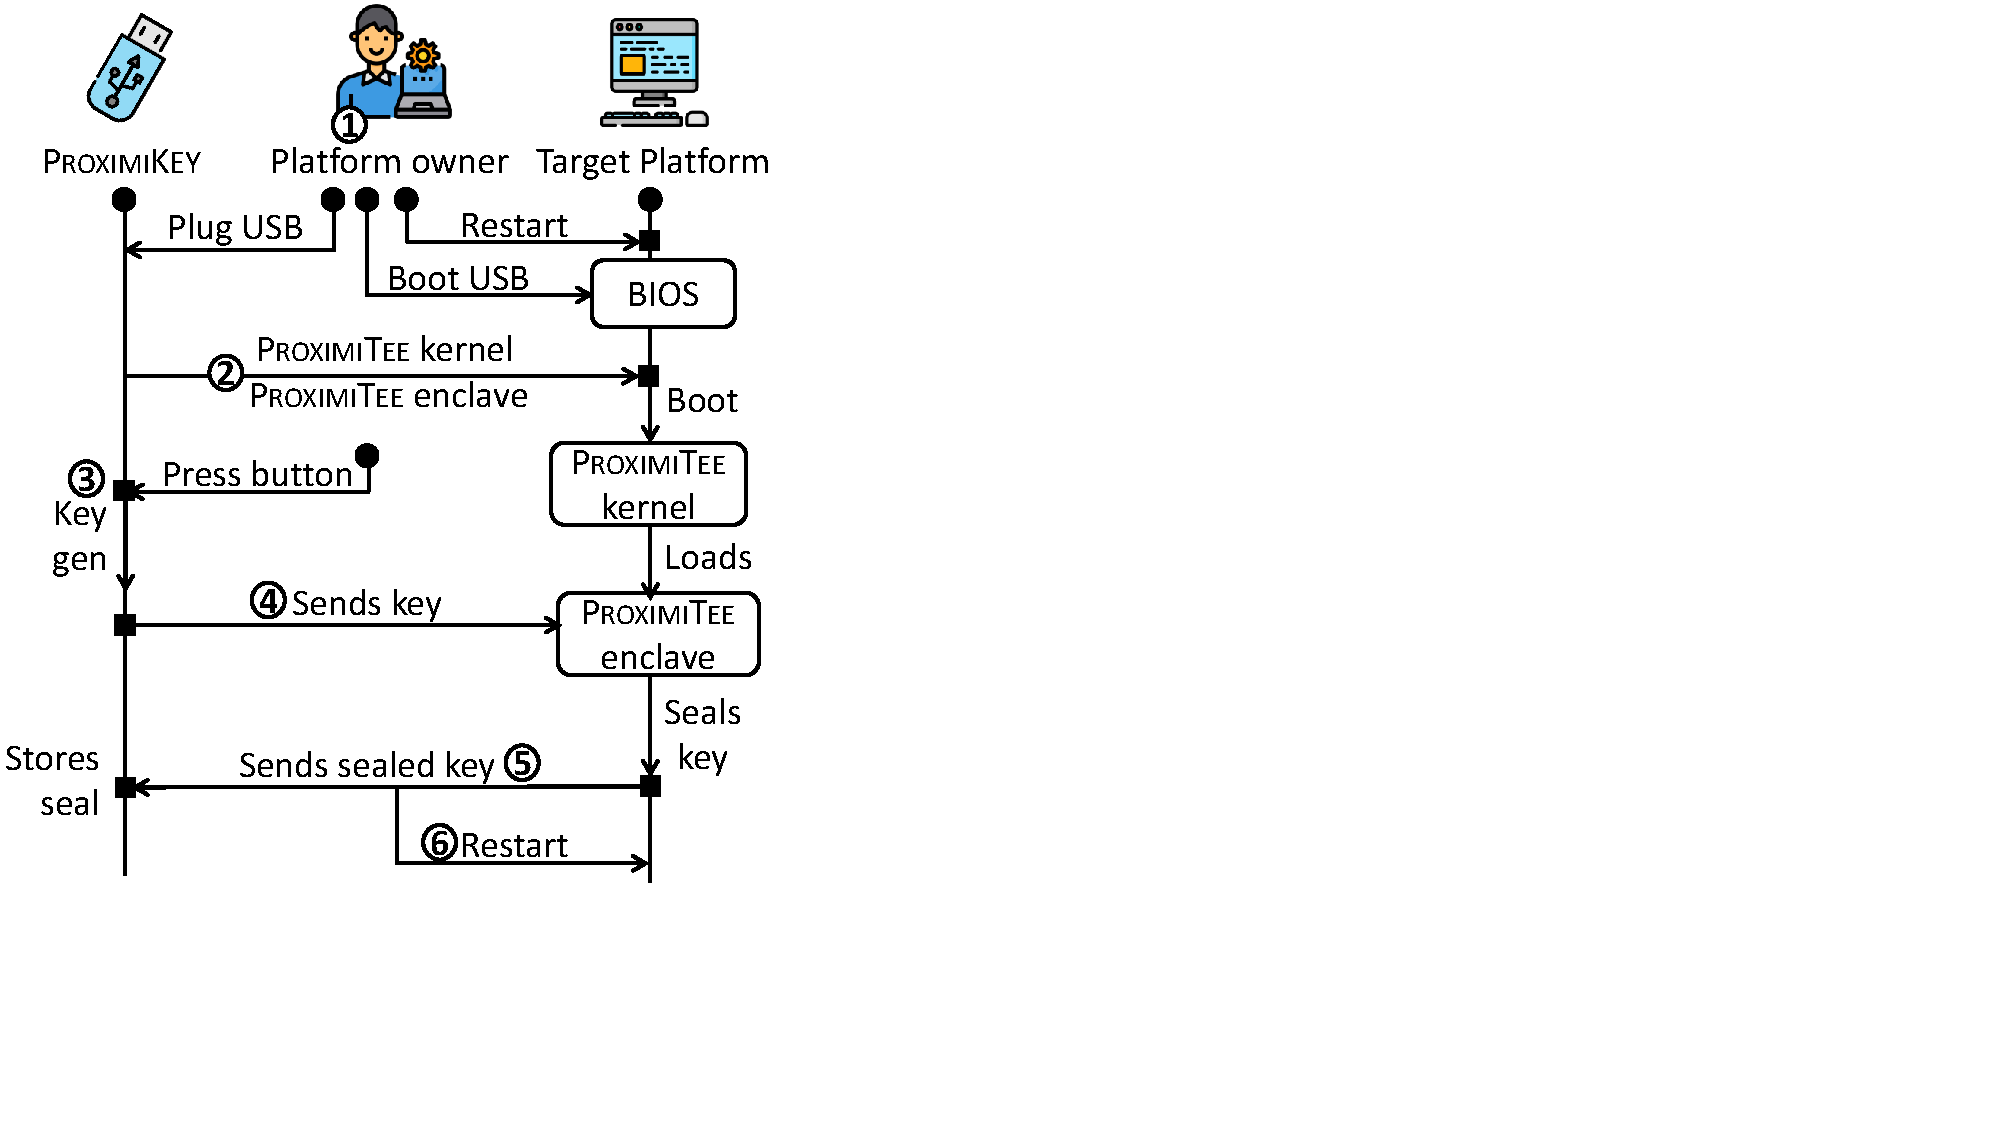
\includegraphics[trim={0 7cm 19cm 0},clip,width=0.75\linewidth]{boot_init.pdf}
 \caption{\textbf{Boot-time initialization.} The \device uses a minimal kernel Linux image to boot and load \nameclave on the target platform and seal a platform specific secret to the \device memory.}
\vspace{-12pt}
 \label{fig:boot-init}
\end{figure}

\else

\begin{figure*}[t!]
    \centering
    \begin{subfigure}[t]{0.5\textwidth}
        \centering
        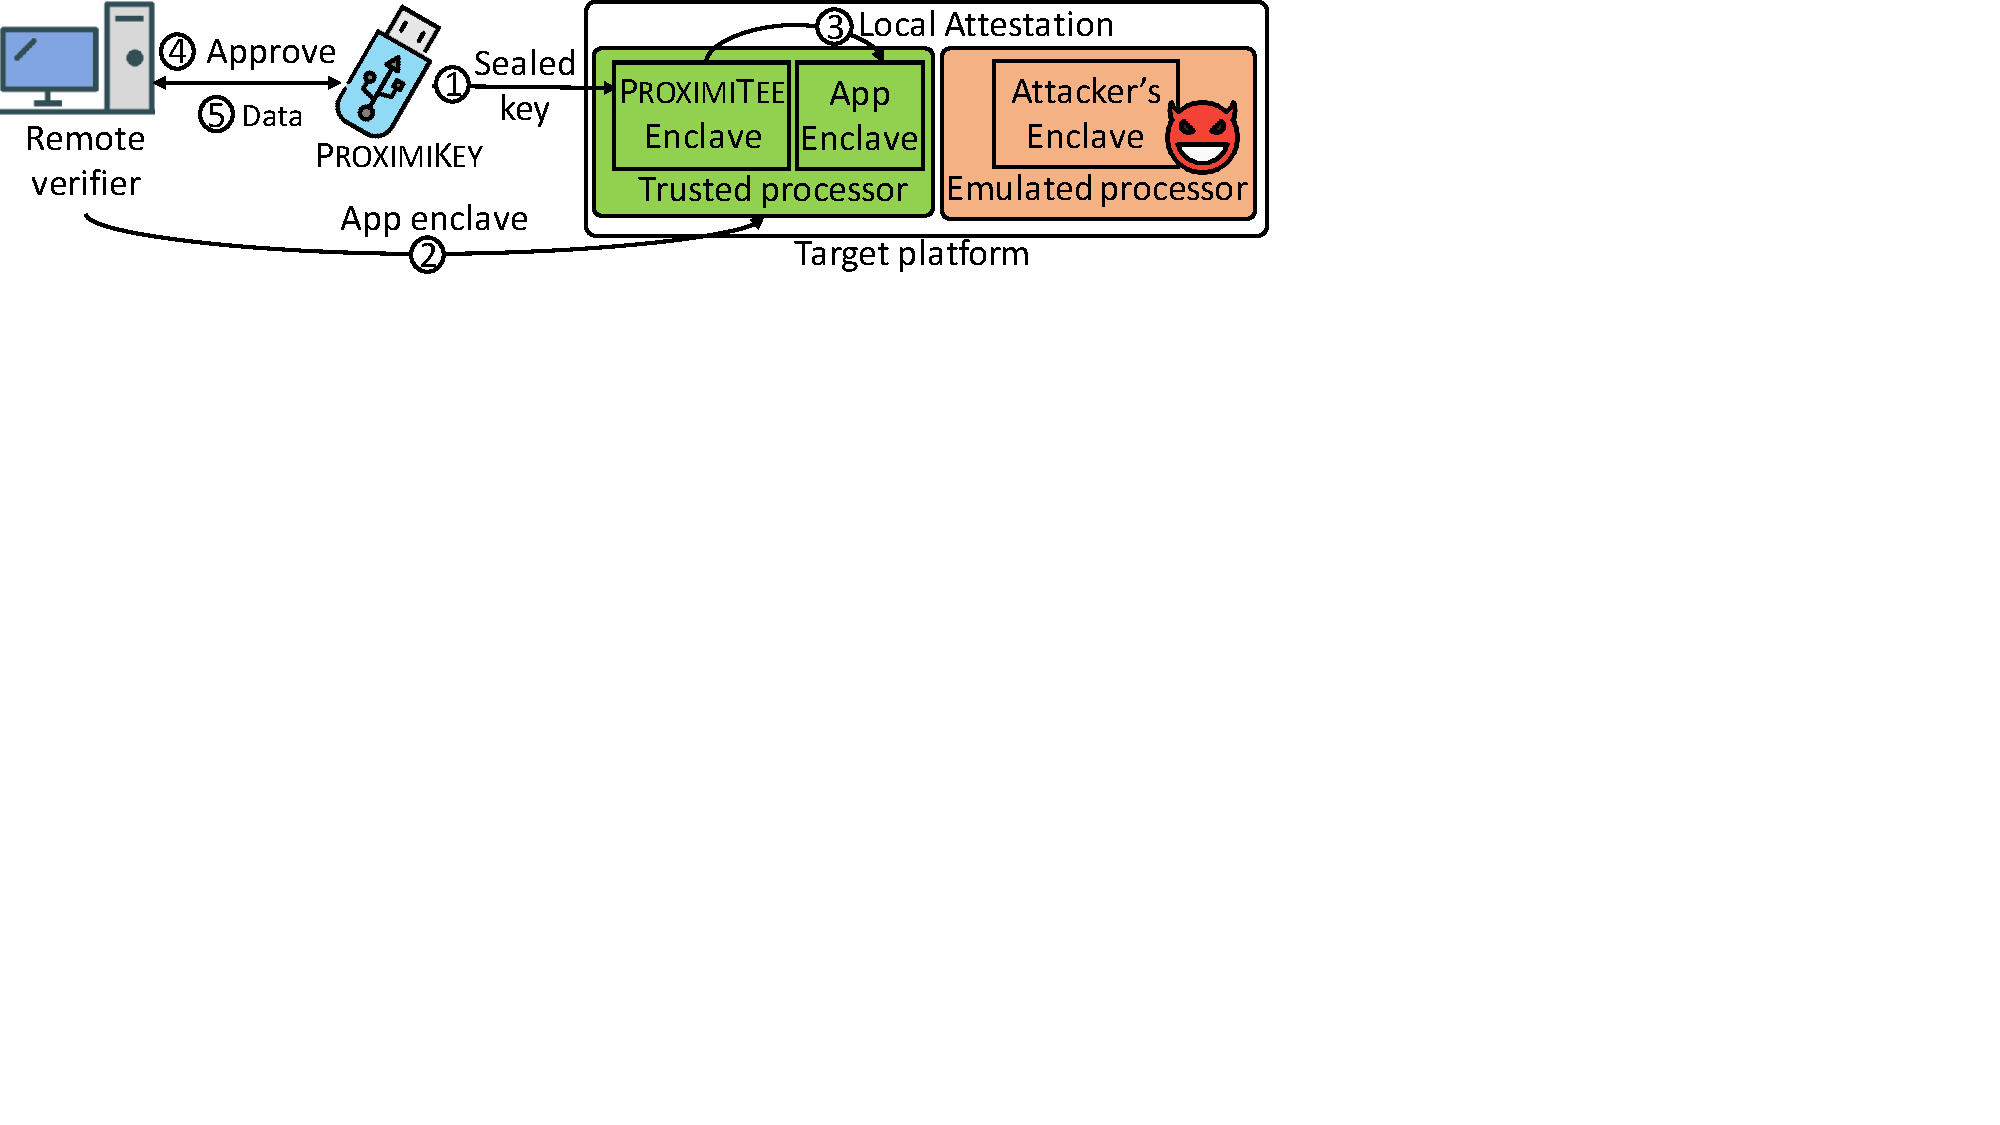
\includegraphics[trim={0 7cm 20cm 0}, clip,  height=2.15in]{boot-attest_1.pdf}
        \caption{\textbf{Flow of the boot-variant attestation.} After the boot-time initialization (refer to Figure~\ref{fig:boot-init}) the \nameclave executes a local attestation with the verifier uploaded \app. }
        \label{fig:boot-attest}
    \end{subfigure}%
    ~ ~~
    \begin{subfigure}[t]{0.5\textwidth}
        \centering
        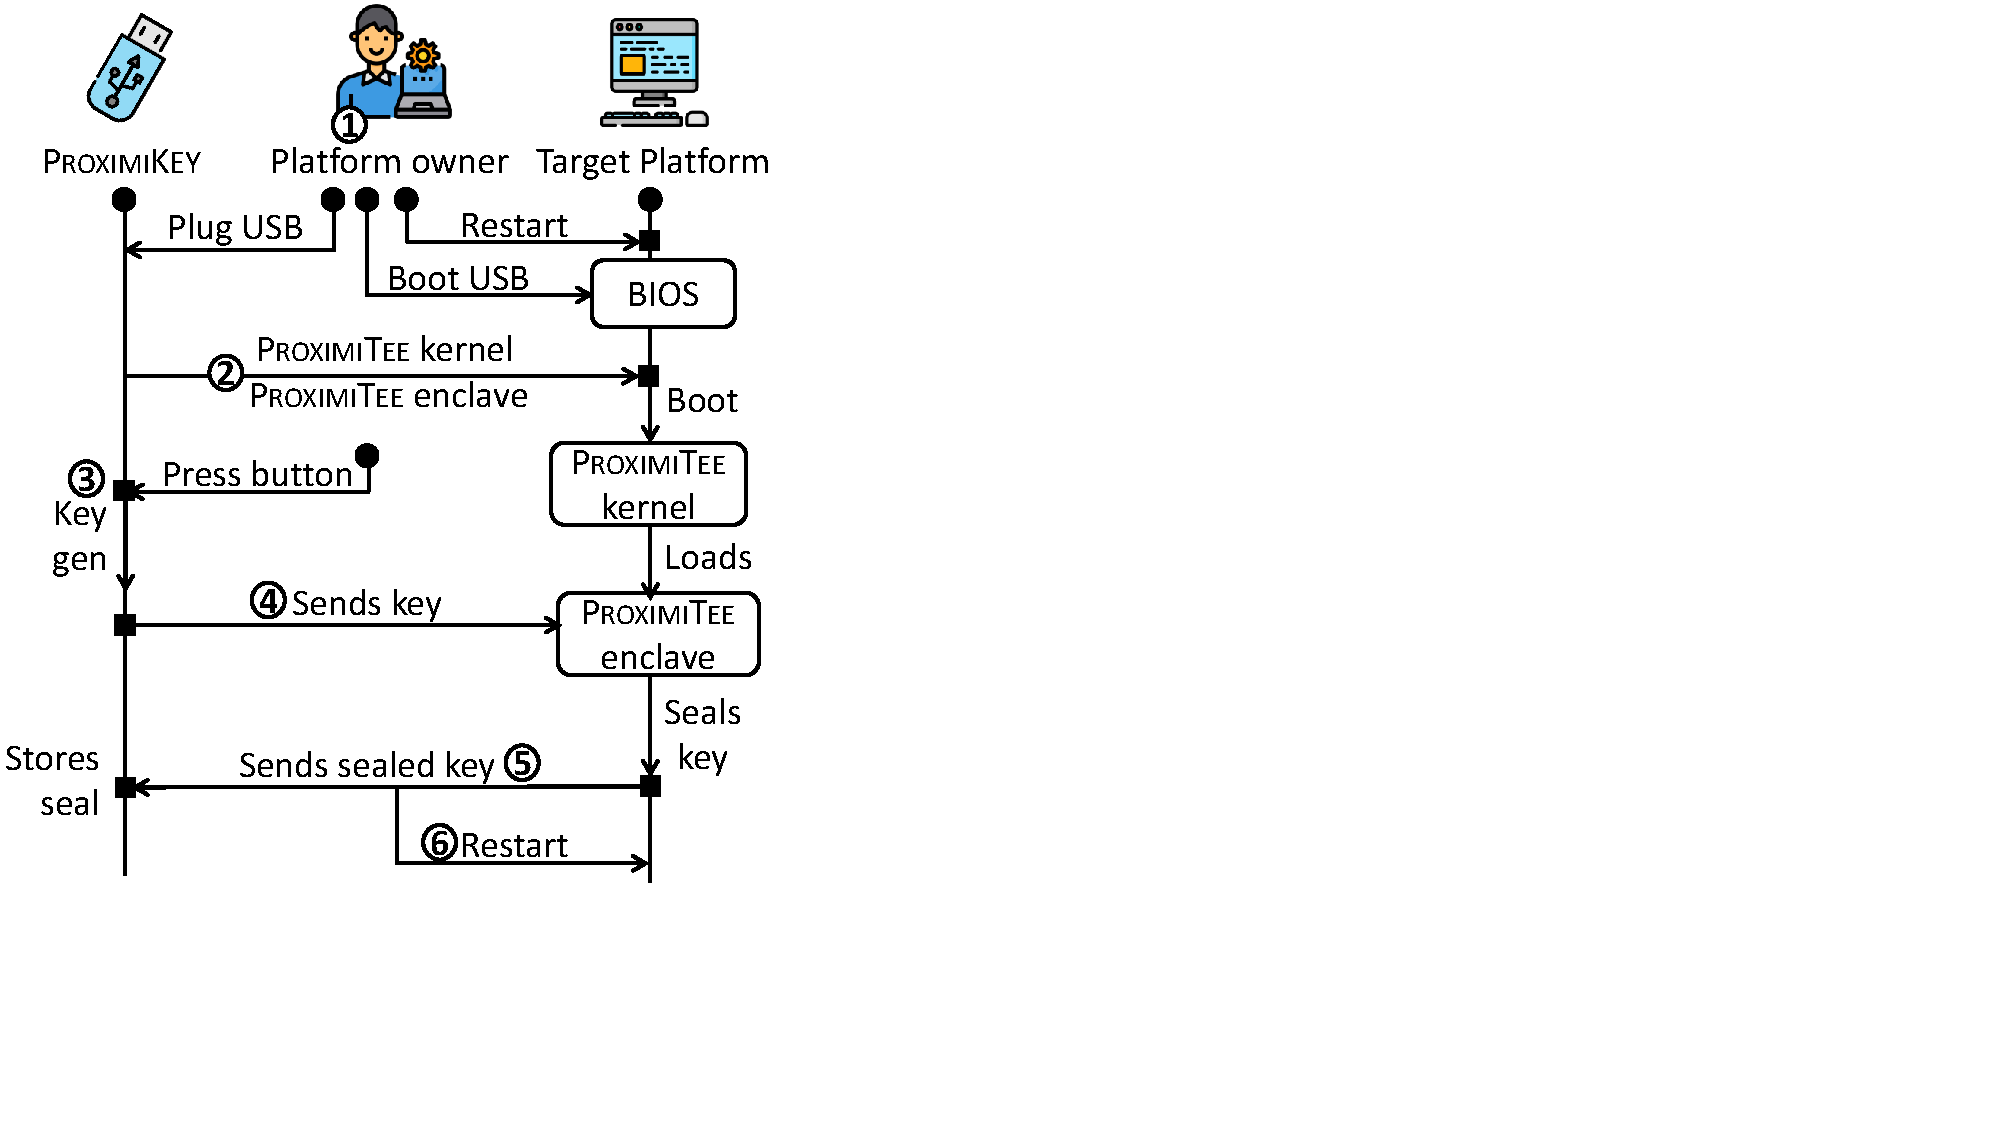
\includegraphics[trim={0 7cm 19cm 0}, clip, height=2.2in]{boot_init.pdf}
        \caption{\textbf{Boot-time initialization.} The \device uses a minimal kernel Linux image to boot and load \nameclave on the target platform and seal a platform specific secret to the \device memory.}
        \label{fig:boot-init}
    \end{subfigure}
    \caption{\textbf{Attestation variant 2: boot-variant attestation.}}
\end{figure*}

\fi



Figure~\ref{fig:boot-attest} illustrates an overview of this solution. During initialization, that is depicted in Figure~\ref{fig:boot-init}, the target platform is booted from the attached \device that loads a minimal \name kernel on the target device. In particular, this kernel includes no network functionality. The kernel starts \name enclave that shares a secret with the device. This shared secret later bootstraps the secure communication between \device and the \name enclave. The security of the bootstrapping relies on the fact that the minimal kernel will not perform enclave emulation at boot time. The \name enclave will later be used as a proxy to attest whether other (application-specific) enclaves in the system are real or emulated and on the same platform.

\ifusenix
\vspace{-15pt}
\else
\fi

\myparagraph{Boot-time initialization.} The boot-time initialization process is performed only once.
This process is depicted in Figure~\ref{fig:boot-init} and it proceeds as follows:



\begin{mylist}
  \item[\one] The platform owner plugs \device to the target platform, restarts it to BIOS and selects the option to boot from \device.
  \item[\two] \device loads the \name kernel and boots from it. The \name kernel starts the \nameclave.
  \item[\three] The user presses a button on \device to confirm that this is a boot-initialization process. This step is necessary to prevent an attack where the compromised OS emulates a system boot.
  \item[\four] \device sends a randomly generated key $\mathcal{K}$ to the \nameclave.
  \item[\five] The enclave returns the sealed key $\mathcal{S}$ corresponding to the key $\mathcal{K}$ ($\mathcal{S}\leftarrow\texttt{Seal}(\mathcal{K})$) to \device that stores the key and the seal pair $(\mathcal{K}, \mathcal{S})$ on its flash storage.
  \item[\six] \device blocks further initializations, sends a restart signal and boots the platform with the normal OS.
\end{mylist}

\ifusenix
\vspace{-15pt}
\else
\fi
\myparagraph{Attestation process.} After initialization the target platform runs a regular OS. The attestation process is depicted in Figure~\ref{fig:boot-attest} and proceeds as follows:

\begin{mylist}

  %\item[\circled{0}] The \device executes aforementioned \name boot-time initialization protocol.

  \item[\one] \device sends the seal $\mathcal{S}$ to the \nameclave that unseals it and retrieves the key $\mathcal{K}$. \device and the \nameclave establish a secure channel (\tls) using $\mathcal{K}$.

  \item[\two] The remote verifier uploads a new \app on the target platform.

  \item[\three] The \nameclave performs local attestation (cf.~Appendix~\ref{sec:background}) on the \app that binds its public key to the attestation. %The local attestation ensures that i) the \app is on the same physical platform, and ii) the code integrity of the \app.

  \item[\four] The \nameclave sends the measurement and the public key of the \app to \device. \device establishes a secure channel to the \app and sends the measurement of the enclave to the remote verifier. The remote verifier then approves the communication to the \app.

  \item[\five] The remote verifier checks that the measurement of the \app is as expected. If this is the case, it can communicate with the enclave through \device.
  %s between the \device and \nameclave and the \nameclave and the \app. \todo{Why go through \nameclave every time?}

\end{mylist}

\ifusenix
\vspace{-15pt}
\else
\fi
\myparagraph{Following communication.} Similar to our previous variant, after the initial attestation all the communication between a remote verifier and the enclave is mediated by the \device that periodically checks the proximity of the attested enclave and terminates the communication channel in case the embedded device is detached.
